\chapter{Neural Networks and Deep Learning}

%%%%
\section{Introduction to Deep Learning}
机器学习本质上就是训练模型来完成\textbf{从输入到输出($\bm{X\to Y}$)的映射}。例如, 给定一张猫的照片, 机器学习模型可以输出``这是一只猫''的结论。

深度学习有3大要点:
\begin{itemize}	
    \item Data
    \item Computation
    \item Algorithms
\end{itemize}

Data可以分为Structured Data和Unstructured Data。Structured Data是指有固定格式的数据, 例如表格、数据库等。Unstructured Data是指没有固定格式的数据, 例如图片、音频、视频等。

Computation是指计算机的计算能力, 例如CPU、GPU、TPU等。

Algorithms是指算法, 例如Logistic Regression、SVM、Neural Networks等。

%%%%
\section{Neural Networks Basics}

表 \ref{tab:notations} 是本章用到的符号说明。为方便起见,所有的向量符号不会加粗,用小写字母表示;同时也不对偏导数进行专门的区分,仍使用$\d $符号表示偏微分。

\begin{table}[htb!]
    \centering
    \begin{threeparttable}
    %%
    \caption{Notations}
    %
    \begin{tabular}{clcc}
        \hline
                                    & \textbf{Notation}                                     & \textbf{Description} & \textbf{Meaning}                                                   \\ \hline
        \multirow{5}{*}{Sizes}      & $m$                                                   & value                & 样本容量                                                               \\
                                    & $n_x$ / $n_h^{[0]}$                                   & value                & 单个样本的特征数(输入层节点数)                                         \\
                                    & $n_y$ / $n_h^{[L]}$                                   & value                & 单个样本的标签数(输出层节点数)                                      \\
                                    & $n_h^{[l]}$ / $n^{[l]}$                               & value                & 第$l$层的神经元个数(隐藏层节点数)                                   \\
                                    & $L$                                                   & value                & 神经网络的层数                                                         \\ \hline
        \multirow{11}{*}{Objects}   & $x^{(i)} \in \mathbb{R}^{n_x}$                        & vector               & 第$i$个样本数据                                                          \\
                                    & $X / A^{[0]} \in {\mathbb{R}^{n_x \times m}}$         & matrix               & 输入矩阵                                                               \\
                                    & $a^{[l](i)} \in \mathbb{R}^{n^{l}}$                   & vector               & 第$i$个样本在第$l$层节点的输出                                                  \\
                                    & $a_j^{[l]} \in \mathbb{R}^{1 \times {m}}$             & vector               & 第$l$层第$j$个节点的输出                                                         \\
                                    & $A^{[l]} \in \mathbb{R}^{n^{[l]} \times {m}}$         & matrix               & 第$l$层节点的输出矩阵                                                         \\
                                    & $y^{(i)} \in \mathbb{R}^{n_y}$                        & vector               & 第$i$个样本的标签                                                         \\
                                    & $Y \in {\mathbb{R}^{n_y \times m}}$                   & matrix               & 样本标签矩阵                                                           \\									
                                    & $\hat{y}^{(i)} \in \mathbb{R}^{n_y}$                  & vector               & 第$i$个样本的标签预测值向量                                                \\
                                    & $\hat{Y} / A^{[L]} \in {\mathbb{R}^{n_y \times m}}$   & matrix               & 标签预测值矩阵($n_y=1$时退化为行向量$\hat{y}$)   						\\
                                    & $W^{[l]} \in \mathbb{R}^{n^{[l]} \times n^{[l-1]}}$   & matrix               & 第$l$层的权重矩阵                                                               \\
                                    & $b^{[l]} \in \mathbb{R}^{n^{[l]}}$                    & vector               & 第$l$层的标签偏置值向量                                                        \\\hline
        \multirow{5}{*}{Other}      & $g^{[l]}(z)$                                          & function             & 第$l$层的激活函数                                                         \\
                                    & $L^{(i)}(\hat{y}^{(i)}, y^{(i)})$                     & function             & 第$i$个样本的代价函数                                                         \\
                                    & $J(X,W,b,Y)$ or $J(\hat{Y},Y)$                        & function             & 代价函数                                                                        \\
                                    & $\alpha$								                & value                & 学习率                                                                        \\
                                    & $\d \mathrm{var}$                              & differential         & 代价函数对变量$\mathrm{var}$的偏微分,即${\partial J}/{\partial \mathrm{var}}$ \\ \hline
    \end{tabular}
    %
    \label{tab:notations} %
    \begin{tablenotes}
        \item[*] 通常情况下$(i)$表示第$i$个样本,而$[l]$表示第$l$层。
    \end{tablenotes}
    %%
    \end{threeparttable}
\end{table}

%%%
\subsection{Binary Classification}
\textbf{二元分类模型}的输入是一个样本$x^{(i)} \in \mathbb{R}^{n_x}$,输出是一个标签$y^{(i)} \in \{0, 1\}$,即$y^{(i)}$只能取0或1且$n_y=1$,对每一个样本得出是或否的结论。

%%%
\subsection{Logistic Regression}
\index{Logistic Regression}

在本节中,由于只考虑一个单层单节点的神经网络,因此省略上标$[l]$,使用简化后的符号如表 \ref{tab:notations_LR} 所示。

\begin{table}[htb!]
    \centering
    \begin{threeparttable}
    \caption{Notations in Logistic Regression}
    \begin{tabular}{clcc}
        \hline
                                    & \textbf{Notation}                         & \textbf{Description} & \textbf{Meaning}                                                   \\ \hline
        \multirow{2}{*}{Sizes}      & $m$                                       & value                & 样本容量                                                               \\
                                    & $n_x$                                     & value                & 单个样本的特征数(输入层节点数)                                         \\ \hline
        \multirow{8}{*}{Objects}    & $x^{(i)} \in \mathbb{R}^{n_x}$            & vector               & 第$i$个样本数据                                                          \\
                                    & $X \in {\mathbb{R}^{n_x \times m}}$       & matrix               & 输入矩阵                                                               \\
                                    & $a^{(i)} / y^{(i)}$                       & binary               & 第$i$个样本的标签实际值                                                        \\
                                    & $y \in \mathbb{R}^{m}$					& vector               & 标签实际值向量                                                          \\
                                    & $\hat{y}^{(i)}$                           & binary               & 第$i$个样本的标签预测值                                                  \\
                                    & $\hat{y} \in {\mathbb{R}^{m}}$            & vector               & 标签预测值向量   					                                     \\
                                    & $w \in \mathbb{R}^{n_x}$                  & vector               & 权重向量                                                                \\
                                    & $b$                                       & value                & 标签偏置值                                                            \\ \hline
        \multirow{2}{*}{Other}      & $J(x,w,b,y)$ or $J(\hat{y},y)$            & function             & 代价函数                                                               \\
                                    & $\d \mathrm{var}$                  & differential         & 代价函数对变量$\mathrm{var}$的偏微分                                    \\ \hline
    \end{tabular}
    \label{tab:notations_LR}
    \end{threeparttable}
\end{table}

对于二元分类模型,相关公式如下:
\begin{equation}
    \hat{y}^{(i)} = \sigma(w^\mathrm{T} x^{(i)} + b) \label{eq:logistic}
\end{equation}
其中sigmoid函数$\sigma(z)$定义为:
\begin{equation}
    \sigma(z) = \frac{1}{1 + \mathrm{e}^{-z}} \label{eq:sigmoid}
\end{equation}
该函数可以把实数域$\mathbb{R}$映射到区间$(0, 1)$,可作为激活函数使用,如图 \ref{fig:sigmoid} 所示。而$z = w^\mathrm{T} x + b$为线性函数,$w$为权重(weight),$b$为偏置(bias)。
\begin{figure}[h!b]
    \centering
    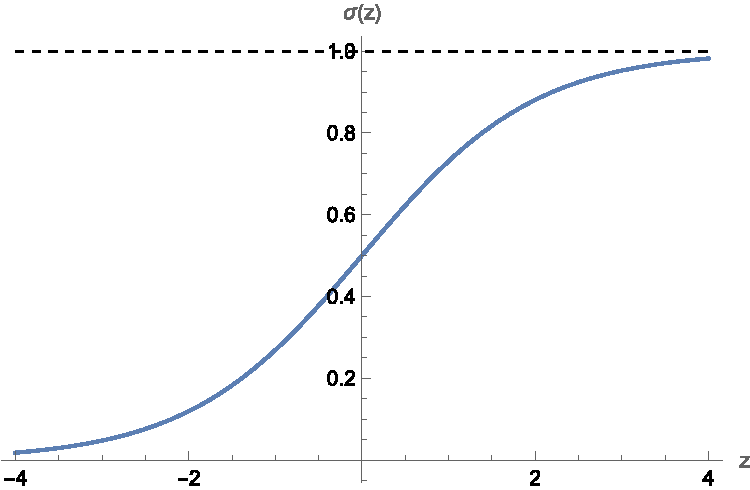
\includegraphics[width=8cm]{sigmoid.pdf}
    \caption{Sigmoid 函数,关于点(0, 0.5)对称}
    \label{fig:sigmoid}
\end{figure}

对某一个样本而言,交叉熵形式的 Loss function(误差函数)定义为:\index{Loss Function}
\begin{equation}
    L(\hat{y}^{(i)}, y^{(i)}) = -\left[y^{(i)} \log \hat{y}^{(i)} + (1 - y^{(i)}) \log (1 - \hat{y}^{(i)})\right] \label{eq:loss}
\end{equation}
该函数与方差类似,当样本的误差越大,Loss function的值越大,如图 \ref{fig:loss} 所示。
\begin{figure}[h!b]
    \centering
    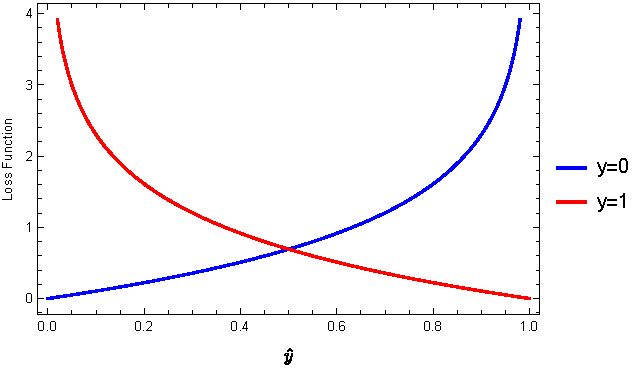
\includegraphics[width=8cm]{LossFunction.pdf}
    \caption{Loss Function 误差函数}
    \label{fig:loss}
\end{figure}

对整个模型而言,Cost function(代价函数/损失函数)定义为:\index{Cost Function}
\begin{equation}
    \begin{aligned}
        J(w, b) &\triangleq  \frac{1}{m} \sum_{i=1}^{m} L(\hat{y}^{(i)}, y^{(i)}) \\
        &= -\frac{1}{m} \sum_{i=1}^{m} \left[y^{(i)} \log \hat{y}^{(i)} + (1 - y^{(i)}) \log (1 - \hat{y}^{(i)})\right] \label{eq:cost}
    \end{aligned}
\end{equation}
相当于误差函数的平均值。

%%%
\subsection{Gradient Descent}
\index{Gradient Descent}

训练过程使用\textbf{梯度下降(Gradient Descent)算法},即:
\begin{equation}
    \mathrm{var} = \mathrm{var} - \alpha \frac{\d J}{\d \mathrm{var}} \label{eq:gradient}
\end{equation}

其中$\mathrm{var}$为一个需要调整的参数,$\alpha$为学习率(Learning Rate)。对于Logistic Regression,梯度下降算法的表达式为:
\begin{equation}
    \begin{aligned}
    w &:= w - \alpha \frac{\d J}{\d w} \\
    b &:= b - \alpha \frac{\d J}{\d b}
    \end{aligned} 
    \label{eq:gradient_logistic}
\end{equation}
其中$:=$表示赋值,通过不断更新$w$, $b$的值使$J$尽可能小。下面介绍具体实现

对于一个样本,有
\begin{equation}
    \begin{aligned}
    z &= w^\mathrm{T} x^{(i)} + b \\
    \hat{y}^{(i)} &= \sigma(z) \\
    L(\hat{y}^{(i)}, y^{(i)}) &= -\left[y^{(i)} \log \hat{y}^{(i)} + (1 - y^{(i)}) \log (1 - \hat{y}^{(i)})\right]
    \end{aligned} 
    \label{eq:gradient_logistic_sample}
\end{equation}
进行求导($x$, $y$均为常量),有
\begin{equation}
    \begin{aligned}
    &\frac{\d L}{\d \hat{y}^{(i)}} = -\frac{y^{(i)}}{\hat{y}^{(i)}} + \frac{1 - y^{(i)}}{1 - \hat{y}^{(i)}} \\
    &\frac{\d \hat{y}^{(i)}}{\d z} = \frac{\mathrm{e}^{-z}}{(1 + \mathrm{e}^{-z})^2} = \frac{1}{1 + \mathrm{e}^{-z}}(1 - \frac{1}{1 + \mathrm{e}^{-z}}) = \hat{y}^{(i)}(1 - \hat{y}^{(i)})\\
    \end{aligned}
\end{equation}
用链式法则,有
\begin{equation}
    \frac{\d L}{\d z} = \frac{\d L}{\d \hat{y}^{(i)}} \frac{\d \hat{y}^{(i)}}{\d z} = (-\frac{y^{(i)}}{\hat{y}^{(i)}} + \frac{1 - y^{(i)}}{1 - \hat{y}^{(i)}})\hat{y}^{(i)}(1 - \hat{y}^{(i)}) = \hat{y}^{(i)} - y^{(i)}
\end{equation}
进而有
\begin{equation}
    \begin{aligned}
    \frac{\d L}{\d w_j} &= \frac{\d L}{\d z} \frac{\d z}{\d w_j} = x_j^{(i)} (\hat{y}^{(i)} - y^{(i)}) \quad (1 \leqslant j \leqslant n_x) \\
    \frac{\d L}{\d b} &= \frac{\d L}{\d z} \frac{\d z}{\d b} = \hat{y}^{(i)} - y^{(i)}
    \end{aligned}
\end{equation}

对于整个训练集,在一个循环中我们对每一个样本都进行一次梯度下降,并对所有样本的梯度进行平均,有
\begin{equation}
    \begin{aligned}
        \frac{\d J}{\d w_j} &= \frac{1}{m} \sum_{i=1}^{m} \frac{\d L}{\d w_j} = \frac{1}{m} \sum_{i=1}^{m} x_j^{(i)} (\hat{y}^{(i)} - y^{(i)}) \quad (1 \leqslant j \leqslant n_x)\\
        \frac{\d J}{\d b} &= \frac{1}{m} \sum_{i=1}^{m} \frac{\d L}{\d b} = \frac{1}{m} \sum_{i=1}^{m} (\hat{y}^{(i)} - y^{(i)})
    \end{aligned}
\end{equation}
得到梯度的平均值后,再进行参数更新,即
\begin{equation}
    \begin{aligned}
    w_j &:= w_j - \alpha \frac{\d J}{\d w} \quad (1 \leqslant j \leqslant n_x) \\
    b &:= b - \alpha \frac{\d J}{\d b}
    \end{aligned} 
\end{equation}
这样就完成了一轮梯度下降的循环。重复多次梯度下降,直到$J$收敛或达到最大迭代次数,就得到了最终的$w$, $b$。

%%%
\subsection{Vectorization}

一个重要的原则是,在训练过程中要避免使用循环,而是使用向量化的方法。向量化可以调用并行计算,相对于循环的串行计算效率更高。\\
要完成下面的矩阵操作,
\begin{equation}
    Z =
    \begin{bmatrix}
        z^{(1)} & z^{(2)} & \cdots & z^{(m)}
    \end{bmatrix}
    = w^\mathrm{T} X + 
    \begin{bmatrix}
        b & b & \cdots & b
    \end{bmatrix}
\end{equation}
可以使用下面的代码
\begin{python}
import numpy as np
# define X, Y, w, b
Z = np.dot(w.T, X) + b
\end{python}
同理,要实现
\begin{equation}
    \begin{aligned}
        \frac{\d J}{\d w_j} &= \frac{1}{m} \sum_{i=1}^{m} \frac{\d L}{\d w_j} = \frac{1}{m} \sum_{i=1}^{m} x_j^{(i)} (\hat{y}^{(i)} - y^{(i)}) \quad (1 \leqslant j \leqslant n_x)\\
        \frac{\d J}{\d b} &= \frac{1}{m} \sum_{i=1}^{m} \frac{\d L}{\d b} = \frac{1}{m} \sum_{i=1}^{m} (\hat{y}^{(i)} - y^{(i)})
    \end{aligned}
\end{equation}
可以继续使用下面的代码
\begin{python}
def sigmoid(x):
    s = 1 / (1 + np.exp(-x))
    return s


A = sigmoid(Z)
dZ = A - Y
dw = np.dot(X, dZ.T) / m
# sum along the column
db = np.sum(dZ, axis=1) / m
# sum will get a row vector regardless of the axis parameter, so we need to reshape it
db = db.reshape(ny, 1)
\end{python}
\verb|np.sum()| 函数的 \verb|axis| 参数表示沿着哪个维度进行求和,\verb|axis=0| 表示沿着列求和,\verb|axis=1| 表示沿着行求和。

在 \verb|numpy| 中,矩阵的维度扩充与 \verb|matlab| 类似,可以自动扩充,也可以使用 \verb|reshape| 函数进行扩充。

矩阵(或向量)在保存时,使用了两重方括号,例如 \verb|[[1, 2], [3, 4]] / [[3, 6, 9]]|,而数组仅有一重方括号,例如 \verb|[1, 2, 3, 4]|。
要把数组转换为向量,可以使用 \verb|reshape()| 函数,例如
\begin{python}
A = np.array([1, 2, 3, 4])
print(A)
print(A.shape)
print(A.T)
A = A.reshape(1, 4)
print(A)
print(A.shape)
print(A.T)
\end{python}
输出结果为
\begin{python}
# array, rank=1
[1 2 3 4]
(4,) 
[1 2 3 4]
# vector
[[1 2 3 4]]
(1, 4) 
[[1]
 [2]
 [3]
 [4]]
\end{python}
\verb|reshape()| 是一个$\mathrm{O}(1)$的操作,不会影响程序的运行效率。在本课程中不要使用 \verb|rank 1 array|,因为它的维度不是$(n, 1)$或$(1, n)$,在进行矩阵运算时会出现错误。

为了确保矩阵的维度正确,可以使用 \verb|assert()| 函数,例如
\begin{python}
assert(A.shape == (1, 4))
\end{python}
如果 \verb|A.shape| 不等于 \verb|(1, 4)|,则会报错。

%%%
\subsection{Explanation of logistic regression cost function}

对于二元分类模型,我们期望$\hat{y}$尽可能接近$y$,即${y}^{(i)}$等于$1$时,$\hat{y}^{(i)}$接近$1$,而${y}^{(i)}$等于$0$时,$\hat{y}^{(i)}$接近$0$。

当$y^{(i)}=1$时,得到正确分类的概率为$\hat{y}^{(i)}$;而当$y^{(i)}=0$时,得到正确分类的概率为$1-\hat{y}^{(i)}$。因此,对于第$i$个样本,可以使用下面的公式来表示这个概率:
\begin{equation}
    P(y^{(i)} | x^{(i)}; w, b) = (\hat{y}^{(i)})^{y^{(i)}} (1-\hat{y}^{(i)})^{1-y^{(i)}}
\end{equation}
假如各个样本是独立的,那么所有样本得到正确分类的概率为
\begin{equation}
    \begin{aligned}
        P(y | x; w, b) &= \prod_{i=1}^{m} P(y^{(i)} | x^{(i)}; w, b)\\
        &= \prod_{i=1}^{m} (\hat{y}^{(i)})^{y^{(i)}} (1-\hat{y}^{(i)})^{1-y^{(i)}}
    \end{aligned}
\end{equation}
为了避免使用累乘和指数运算,可以在等式两边取对数,得到
\begin{equation}
    \begin{aligned}
        \log P(y | x; w, b) &= \sum_{i=1}^{m} \log (\hat{y}^{(i)})^{y^{(i)}} (1-\hat{y}^{(i)})^{1-y^{(i)}}\\
        &= \sum_{i=1}^{m} \left[ y^{(i)} \log \hat{y}^{(i)} + (1-y^{(i)}) \log (1-\hat{y}^{(i)}) \right]
    \end{aligned}
\end{equation}
习惯上等式右边要取平均值进行归一化,因此可以得到
\begin{equation}
    \frac{1}{m} \log P(y | x; w, b) = \frac{1}{m} \sum_{i=1}^{m} \left[ y^{(i)} \log \hat{y}^{(i)} + (1-y^{(i)}) \log (1-\hat{y}^{(i)}) \right]
\end{equation}
我们期望这个值越大越好,为了使用梯度下降法,可以对上式取负号,得到
\begin{equation}
    J(w, b) = - \frac{1}{m} \sum_{i=1}^{m} \left[ y^{(i)} \log \hat{y}^{(i)} + (1-y^{(i)}) \log (1-\hat{y}^{(i)}) \right]
\end{equation}
这就是代价函数的定义。我们期望代价函数的值越小越好,因此可以使用梯度下降法来求解$w$和$b$。

%%%%
\section{Shallow Neural Networks}
\begin{wenxintishi}
    在上一节中,我们构建的模型本质上是一个单节点的一层神经“网络”。在本节中,我们将构建一个两层的神经网络,也就是一个\textbf{浅层神经网络(Shallow Neural Network)}。
\end{wenxintishi}

%%%
\subsection{Neural Networks Representation}

神经网络是若干“层”(Layer)的组合,每一层都是若干“节点”(Node)的组合。第一层为“输入层”(Input Layer),最后一层为“输出层”(Output Layer),中间的层为“隐藏层”(Hidden Layer)。在计数时,通常将输入层记为第$0$层,隐藏层从第$1$层开始计数。

隐藏层和输出层都是全连接层,每个节点都与上一层的所有节点相连。隐藏层和输出层的节点都是\textbf{神经元(Neuron)},每个神经元都有一个\textbf{激活函数(Activation Function)},用来计算该神经元的输出。隐藏层和输出层的激活函数可以不同,但是通常情况下都是相同的。

浅层神经网络具有$1$个输入层、$1$个隐藏层、$1$个输出层,其结构如图 \ref{fig:shallow_nn} 所示,该图展示了第$i$个样本的神经网络结构,每个小写字母表示一个值。实际上,神经网络会同时处理多个样本,执行矩阵运算。

每个节点会进行两个计算,分别是\textbf{线性计算}和\textbf{激活函数计算},如图 \ref{fig:node} 所示。节点首先把上一层的所有节点的输出值乘以权重,然后把所有结果相加,再加上偏置值,得到线性计算的结果$z$。然后把$z$作为激活函数的输入,得到激活函数的输出,作为该节点的输出$a$。$z$可作为一个中间量,与$a$维度相同。

\begin{figure}[h!bt]
    \centering
    \begin{tikzpicture}[x=1.5cm, y=1.5cm, >=stealth]
        \def\nx{3}
        \def\nu{4}
        % 输入层
        \foreach \i in {1,...,\nx}
            \node[circle, draw=none] (x\i) at (0,2-\i) {$x_\i^{(i)}$};
        \foreach \i in {1,...,\nx}
            \node[coordinate] (lx\i) at (0.2,2-\i) {};
        
        % 隐藏层
        \foreach \h in {1,...,\nu}
            \node[circle, draw=blue, fill=white, inner sep=0pt, minimum size=10mm] (h\h) at (2,2.5-\h) {$a_\h^{[1](i)}$};
        
        % 输出层
        \node[circle, draw=yellow, fill=white, inner sep=0pt, minimum size=10mm] (o) at (4,0) {$a^{[2](i)}$};
    
        % 预测值
        \node[circle, draw=none] (yhat) at (5.5,0) {$\hat{y}^{(i)}$};
        
    
        % 连接
        \foreach \i in {1,...,\nx}
            \foreach \h in {1,...,\nu}
                \draw[->, color=base1] (lx\i) -- (h\h);
        
        \foreach \h in {1,...,\nu}
            \draw[->, color=base1] (h\h) -- (o);
        
        \draw[->, color=base1] (o) -- (yhat);
        
        % 标签
        \def\labely{-2}
        \node [green] at (0,2.2) {layer 0};
        \node [blue] at (2,2.2) {layer 1};
        \node [yellow] at (4,2.2) {layer 2};
        \draw [decorate,decoration={calligraphic brace,amplitude=4pt,mirror}] (-0.35,\labely) -- (0.35,\labely) node [green,midway,yshift=-0.5cm] {输入层};
        \draw [decorate,decoration={calligraphic brace,amplitude=4pt,mirror}] (1.3,\labely) -- (2.7,\labely) node [blue,midway,yshift=-0.5cm] {隐藏层};
        \draw [decorate,decoration={calligraphic brace,amplitude=4pt,mirror}] (3.5,\labely) -- (4.5,\labely) node [yellow,midway,yshift=-0.5cm] {输出层};
        \draw [decorate,decoration={calligraphic brace,amplitude=4pt,mirror}] (5.15,\labely) -- (5.85,\labely) node [red,midway,yshift=-0.5cm] {预测值};
    
    \end{tikzpicture}
    \caption{Shallow Neural Network 浅层神经网络}
    \label{fig:shallow_nn}
\end{figure}

\begin{figure}[h!bt]
    \centering
    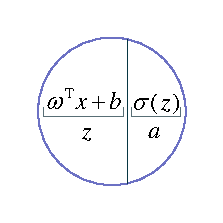
\includegraphics[width=4cm]{node.pdf}
    \caption{单个节点的结构}
    \label{fig:node}
\end{figure}

%%%
\subsection{Activation Functions}
\index{Activation Functions}

常见的激活函数有sigmoid函数、tanh函数、ReLU函数、leaky ReLU函数等,如图 \ref{fig:activation} 所示。对于导数不存在的点,可以使用左导数或右导数代替。

\begin{figure*}[h!bt]
    \centering
    \subfigure[$\mathrm{sigmoid}(z) = \frac{1}{1+\mathrm{e}^{-z}}$]{
        \begin{minipage}[t]{0.45\linewidth}
            \centering
            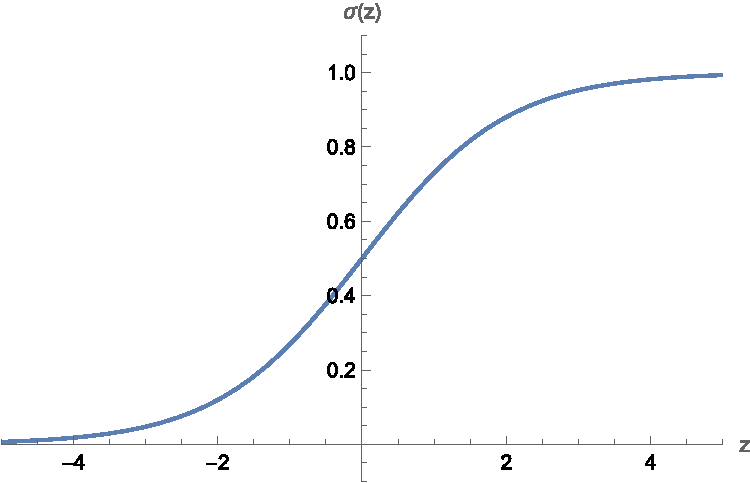
\includegraphics[width=7cm]{activation_sigmoid.pdf}
        \end{minipage}
    }%
    \subfigure[$\mathrm{tanh}(z) = \frac{\mathrm{e}^{z} - \mathrm{e}^{-z}}{\mathrm{e}^{z} + \mathrm{e}^{-z}}$]{
        \begin{minipage}[t]{0.45\linewidth}
            \centering
            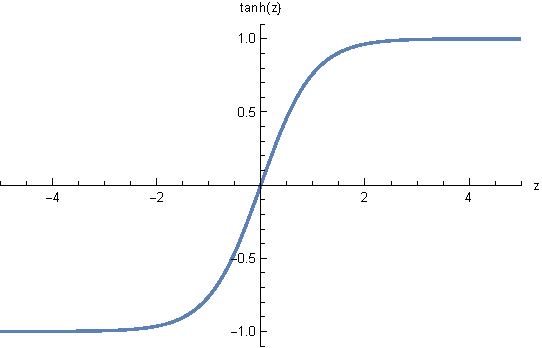
\includegraphics[width=7cm]{activation_tanh.pdf}
        \end{minipage}
    }%
    %此处的空行很重要,想让图片在什么地方换行就在代码对应位置空行

    \subfigure[$\mathrm{ReLU}(z) = \max(0, z)$]{
        \begin{minipage}[t]{0.45\linewidth}
            \centering
            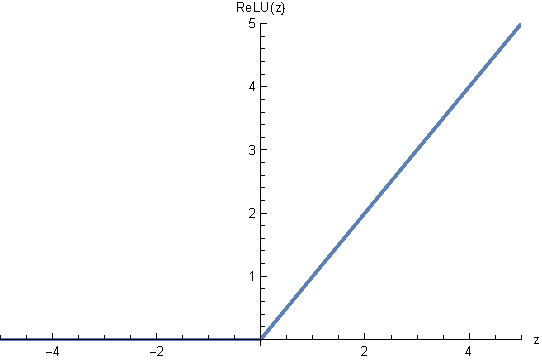
\includegraphics[width=7cm]{activation_ReLU.pdf}
        \end{minipage}
    }%
    \subfigure[$\mathrm{LeakyReLU}(z) = \max(0.01z, z)$]{
        \begin{minipage}[t]{0.45\linewidth}
            \centering
            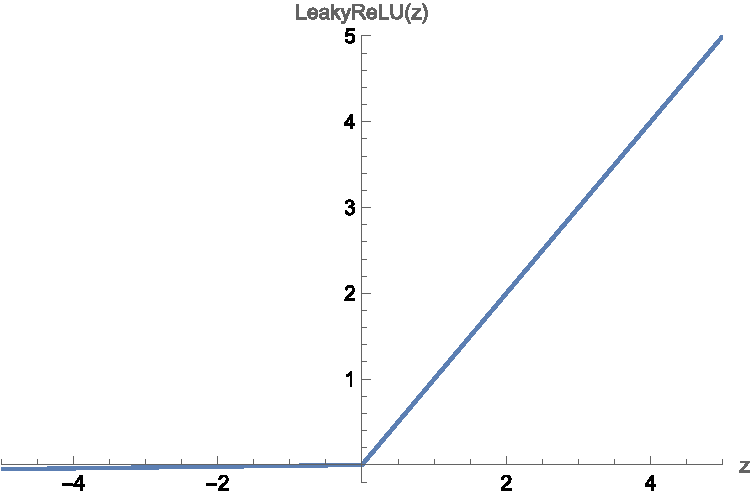
\includegraphics[width=7cm]{activation_LeakyReLU.pdf}
        \end{minipage}
    }%
    \centering
    \caption{Activation Functions 激活函数}
    \label{fig:activation}
\end{figure*}

这些激活函数的导数分别为:
\begin{equation}
    \begin{aligned}
        \frac{\d }{\d z}\mathrm{sigmoid}(z) &= \mathrm{sigmoid}(z)\left(1-\mathrm{sigmoid}(z)\right) \\
        \frac{\d }{\d z}\mathrm{tanh}(z) &= 1 - \mathrm{tanh}^2(z) \\
        \frac{\d }{\d z}\mathrm{ReLU}(z) &= 
            \begin{cases}
                0, &z < 0 \\
                1, &z \geqslant 0
            \end{cases}\\
        \frac{\d }{\d z}\mathrm{LeakyReLU}(z) &= 
            \begin{cases}
                0.01, &z < 0 \\
                1, &z \geqslant 0
            \end{cases}
    \end{aligned}
\end{equation}

需要强调的是,激活函数是必要的,如果没有激活函数,那么神经网络的每一层都是线性的,无论有多少层,整个神经网络都相当于一层线性函数,这样就无法解决复杂的问题。

%%%
\subsection{Gradient Descent for Neural Networks}
在训练整个神经网络时,需要对每一层的权重和偏置进行梯度下降,因此需要对每一层的梯度进行计算。

我们的目标是最小化代价函数$J(W^{[1]}, b^{[1]}, W^{[2]}, b^{[2]}, \cdots, W^{[L]}, b^{[L]})$,其中$L$为神经网络的层数。对于第$l$层,先求出权重和偏置的偏导数,然后再进行梯度下降,即
\begin{equation}
    \begin{aligned}
        W^{[l]} &:= W^{[l]} - \alpha \frac{\d J}{\d W^{[l]}} \\
        b^{[l]} &:= b^{[l]} - \alpha \frac{\d J}{\d b^{[l]}}
    \end{aligned}
\end{equation}

%%%
\subsection{Backpropagation}
\index{Backpropagation}
在神经网络中,梯度下降用到了\textbf{反向传播/后向传播算法(Backpropagation)},该算法的基本思想是,先计算代价函数对输出层的梯度,然后再反向传播到每一层,计算每一层$W$和$b$的梯度。
需要注意,在每一轮梯度下降中,\textbf{所有的$X$, $Y$, $Z$, $A$都是已知的常量,而$W$, $b$是需要更新的}。

在推导过程中,需要补充一些矩阵导数运算的知识,参见附录 \ref{sec:matrix_derivative}。以下过程中使用的符号如表 \ref{tab:notations} 所示。

对于第$l$层,\colorbox{LemonChiffon}{已知$\dfrac{\d J}{\d A^{[l]}}$}和关系\footnote{为了避免一次转置运算,此处的$W$其实是“横放”的,从其行列数可以看出。在上一节中,$w$是作为一个列向量而不是行向量出现的。}
\begin{equation}
    \vcenter{\hbox{\tikzmarknode{Zl}{$Z^{[l]}$}}} \vcenter{\hbox{$\vphantom{1}=\vphantom{1}$\tikzmarknode{Wl}{$W^{[l]}$}\tikzmarknode{Al-1}{$A^{[l-1]}$}$\vphantom{1}+\vphantom{1}$}} \begin{bmatrix} \tikzmarknode[outer ysep=2pt]{bl}{b^{[l]}} & b^{[l]} & \cdots & b^{[l]} \end{bmatrix}_{\substack{\scriptstyle n^{[l]}\times m}}
    \annotate[yshift=1em]{above}{Zl}{$n^{[l]}\times m$}
    \annotate[yshift=-1em]{below,left}{Wl}{$n^{[l]}\times n^{[l-1]}$}
    \annotate[yshift=-1em]{below}{Al-1}{$n^{[l-1]}\times m$}
    \annotate[yshift=1em]{above}{bl}{$n^{[l]}\times 1$}
    \label{eq:backpropagation_known_1}
\end{equation}
\begin{equation}
    \tikzmarknode{Al}{A^{[l]}} = g^{[l]}(\tikzmarknode{Zl2}{Z^{[l]}})
    \vspace{1em}
    \label{eq:backpropagation_known_2}
    \annotatetwo[yshift=-1em]{below,label below}{Al}{Zl2}{$n^{[l]}\times m$}
\end{equation}
\colorbox{LemonChiffon}{要计算$\dfrac{\d J}{\d A^{[l-1]}}$, $\dfrac{\d J}{\d W^{[l]}}$和$\dfrac{\d J}{\d b^{[l]}}$}。
根据结论\eqref{eq:matrix_derivative_conclusion1},式\eqref{eq:backpropagation_known_1}可推出下面的关系
\begin{align}
    \frac{\d J}{\d W^{[l]}} &= \frac{\d J}{\d Z^{[l]}} A^{[l-1] \mathrm{T}} 
    \label{eq:backpropagation_conc_1} \\
    \frac{\d J}{\d A^{[l-1]}} &= W^{[l] \mathrm{T}} \frac{\d J}{\d Z^{[l]}}
    \label{eq:backpropagation_conc_2}
\end{align}
根据结论\eqref{eq:matrix_derivative_conclusion2},式\eqref{eq:backpropagation_known_2}表明
\begin{equation}
    \frac{\d J}{\d Z^{[l]}} = g^{[l]'}(Z^{[l]}) \odot \frac{\d J}{\d A^{[l]}}
    \label{eq:backpropagation_conc_3}
\end{equation}
由于$b^{[l]}$在计算时进行了维度扩充,$\dfrac{\d J}{\d b^{[l]}}$的求取较为特殊。首先考虑第$i$个样本,上面的关系可以写成
\begin{equation}
    z^{[l](i)} = W^{[l]} a^{[l-1](i)} + b^{[l]}
    \label{eq:backpropagation_known_1_sample}
\end{equation}
根据结论\eqref{eq:matrix_derivative_conclusion1},式\eqref{eq:backpropagation_known_1_sample}可推出下面的关系
\begin{equation}
    \frac{\d L^{(i)}}{\d b^{[l]}} = \frac{\d L^{(i)}}{\d z^{[l](i)}}
    \label{eq:backpropagation_known_1_sample_derivative}
\end{equation}
一般认为各个样本间相互独立,从而有
\begin{equation}
    \frac{\d L^{(\textcolor{blue}{i})}}{\d z^{[l](\textcolor{red}{j})}}=0
    , \quad \textcolor{blue}{i} \neq \textcolor{red}{j}, \quad 0 \leqslant l \leqslant L
    \label{eq:backpropagation_known_1_sample_derivative_independent}
\end{equation}
回顾代价函数的定义
\begin{equation}
    J = \frac{1}{m} \sum_{i=1}^{m} L(\hat{y}^{(i)}, y^{(i)})
\end{equation}
结合式\eqref{eq:backpropagation_known_1_sample_derivative_independent},可得
\begin{equation}
    \begin{aligned}
        \frac{\d J}{\d z^{[l](i)}} 
        &= \frac{1}{m}  \sum_{\textcolor{red}{j}=1}^{m} \frac{\d L^{(\textcolor{red}{j})}}{\d z^{[l](i)}} \\
        &= \frac{1}{m}  \left( \sum_{\substack{1 \leqslant \textcolor{red}{j} \leqslant m \\ \textcolor{red}{j} \neq i}} \tikzmarknode{zero}{\frac{\d L^{(\textcolor{red}{j})}}{\d z^{[l](i)}}} + \frac{\d L^{(i)}}{\d z^{[l](i)}} \right) \\
        &= \frac{1}{m} \frac{\d L^{(i)}}{\d z^{[l](i)}} \\
    \end{aligned}
    \annotate[yshift=1em]{above}{zero}{equals 0}
\end{equation}
两边乘$m$即得
\begin{equation}
    \frac{\d L^{(i)}}{\d z^{[l](i)}} = m \frac{\d J}{\d z^{[l](i)}}
\end{equation}
结合式\eqref{eq:backpropagation_known_1_sample_derivative}和代价函数定义,可推知
\begin{equation}
    \begin{aligned}
        \frac{\d J}{\d b^{[l]}} 
        &= \frac{1}{m} \sum_{i=1}^{m} \frac{\d L^{(i)}}{\d b^{[l]}} \\
        &= \frac{1}{m} \sum_{i=1}^{m} \frac{\d L^{(i)}}{\d z^{[l](i)}} \\
        &= \frac{1}{m} \sum_{i=1}^{m} m \frac{\d J}{\d z^{[l](i)}} \\
        &= \tikzmarknode{db}{\sum_{i=1}^{m} \frac{\d J}{\d z^{[l](i)}}}
    \label{eq:backpropagation_conc_4}
    \end{aligned}
    \vspace{2em}
    \renewcommand{\eqnannotationstrut}{\rule[-0.7\baselineskip]{0pt}{1.5\baselineskip}}
    \annotate[yshift=0em]{below}{db}{相当于$\dfrac{\d J}{\d Z^{[l]}}$沿水平方向求和}
    \renewcommand{\eqnannotationstrut}{\strut} % package default
\end{equation}
综合式\eqref{eq:backpropagation_conc_3}, \eqref{eq:backpropagation_conc_2}, \eqref{eq:backpropagation_conc_1}, 和\eqref{eq:backpropagation_conc_4},可得
\footnote{此推导结果与课程不同,主要区别是系数$\dfrac{1}{m}$的位置不同。课程中将$\dfrac{1}{m}$放在了所有的$\dfrac{\d J}{\d W}$和$\dfrac{\d J}{\d b}$处,但实际上应该位于$\dfrac{\d J}{\d A^{[L]}}$处并反向传播至各层。但是这不会影响最终的结果。}
\begin{align}
    \frac{\d J}{\d Z^{[l]}} &= g^{[l]'}(Z^{[l]}) \odot \frac{\d J}{\d A^{[l]}} \\
    \frac{\d J}{\d A^{[l-1]}} &= W^{[l] \mathrm{T}} \frac{\d J}{\d Z^{[l]}} \\
    \frac{\d J}{\d W^{[l]}} &= \frac{\d J}{\d Z^{[l]}} A^{[l-1] \mathrm{T}} \label{eq:dw_real} \\
    \frac{\d J}{\d b^{[l]}} &= \sum_{i=1}^{m} \frac{\d J}{\d z^{[l](i)}} \label{eq:db_real}
\end{align}
将以上结论写成伪代码形式,
\begin{align}
    \mathtt{dZ^{\textcolor{Magenta}{[}l\textcolor{Magenta}{]}}} &= \mathtt{g^{\textcolor{Magenta}{[}l\textcolor{Magenta}{]}'}\textcolor{yellow}{(}Z^{\textcolor{Magenta}{[}l\textcolor{Magenta}{]}}\textcolor{yellow}{)} \,\tikzmarknode[outer ysep=2pt]{star}{*}\, dA^{\textcolor{Magenta}{[}l\textcolor{Magenta}{]}}} \\
    \mathtt{dA^{\textcolor{Magenta}{[}l-\textcolor{green}{1}\textcolor{Magenta}{]}}} &= \mathtt{np.dot\textcolor{yellow}{(}W^{\textcolor{Magenta}{[}l\textcolor{Magenta}{]}}.T, dZ^{\textcolor{Magenta}{[}l\textcolor{Magenta}{]}}\textcolor{yellow}{)}} \\
    \mathtt{dW^{\textcolor{Magenta}{[}l\textcolor{Magenta}{]}}} &= \mathtt{np.dot\textcolor{yellow}{(}dZ^{\textcolor{Magenta}{[}l\textcolor{Magenta}{]}}, A^{\textcolor{Magenta}{[}l-\textcolor{green}{1}\textcolor{Magenta}{]}}.T\textcolor{yellow}{)}} \label{eq:dw} \\
    \mathtt{db^{\textcolor{Magenta}{[}l\textcolor{Magenta}{]}}} &= \mathtt{np.sum\textcolor{yellow}{(}dZ^{\textcolor{Magenta}{[}l\textcolor{Magenta}{]}}, axis=\textcolor{green}{1}, keepdims=\textcolor{blue}{True}\textcolor{yellow}{)}} \label{eq:db}
    \annotate[yshift=1.5em]{above}{star}{element-wise multiplication}
\end{align}
逐元素相乘使用*或 \verb|np.multiply| 均可,区别在于 \verb|np.multiply| 可以进行维度扩充。计算得到的 \verb|dW| 和 \verb|db| 存入 \verb|grads| 字典中,然后使用梯度下降法更新$W$和$b$。

下面来\colorbox{LemonChiffon}{计算$\dfrac{\d J}{\d A^{[L]}}$}。回顾损失函数(交叉熵损失函数)的定义
\begin{equation}
    L^{(i)} = -\left[y^{(i)} \log \hat{y}^{(i)} + (1 - y^{(i)}) \log (1 - \hat{y}^{(i)})\right]
\end{equation}
对其求导,可得
\begin{equation}
    \frac{\d L^{(i)}}{\d \hat{y}^{(i)}} = -\frac{y^{(i)}}{\hat{y}^{(i)}} + \frac{1 - y^{(i)}}{1 - \hat{y}^{(i)}}
\end{equation}
从而
\begin{equation}
    \frac{\d J}{\d \hat{y}^{(i)}} 
    = \frac{1}{m} \sum_{\textcolor{red}{j}=1}^{m} \frac{\d L^{(\textcolor{red}{j})}}{\d \hat{y}^{(i)}} 
    = \frac{1}{m} \frac{\d L^{(i)}}{\d \hat{y}^{(i)}} 
    = \frac{1}{m} \left(-\frac{y^{(i)}}{\hat{y}^{(i)}} + \frac{1 - y^{(i)}}{1 - \hat{y}^{(i)}}\right)
\end{equation}
将各个样本的值写在一起,可得
\begin{equation}
    \frac{\d J}{\d \hat{Y}} 
    = \begin{bmatrix} \dfrac{\d J}{\d \hat{y}^{(1)}} & \dfrac{\d J}{\d \hat{y}^{(2)}} & \cdots & \dfrac{\d J}{\d \hat{y}^{(m)}} \end{bmatrix}
    = \frac{1}{m} \left(-\frac{Y}{\hat{Y}} + \frac{1 - Y}{1 - \hat{Y}}\right)
\end{equation}
即
\begin{equation}
    \frac{\d J}{\d A^{[L]}} 
    = \frac{1}{m} \left(-\frac{Y}{A^{[L]}} + \frac{1 - Y}{1 - A^{[L]}}\right)
\end{equation}
写成伪代码形式为
\begin{equation}
    \mathtt{dA^{\textcolor{Magenta}{[}L\textcolor{Magenta}{]}}} = \mathtt{\textcolor{blue}{(}np.divide\textcolor{yellow}{(}Y, A^{\textcolor{Magenta}{[}L\textcolor{Magenta}{]}}\textcolor{yellow}{)} - np.divide\textcolor{yellow}{(}1 - Y, 1 - A^{\textcolor{Magenta}{[}L\textcolor{Magenta}{]}}\textcolor{yellow}{)}\textcolor{blue}{)}/m} \label{eq:da}
\end{equation}
\textbf{从输出层开始,先得到$\dfrac{\d J}{\d A^{[L]}}$(也就是$\dfrac{\d J}{\d \hat{Y}}$),然后逐层向前计算,直到第$1$层,即可得到所有的梯度。}

\vspace{\baselineskip}
对于本节要构建的浅层神经网络,第一层使用的激活函数为tanh函数,而第二层使用的激活函数为sigmoid函数,
\begin{align}
    A^{[1]} = g^{[1]}(Z^{[1]}) &\quad \Rightarrow \quad g^{[1]'}(Z) = 1-A^{[1]2} \\
    A^{[2]} = g^{[2]}(Z^{[2]}) &\quad \Rightarrow \quad g^{[2]'}(Z) = A^{[2]}(1-A^{[2]})
\end{align}
利用
\begin{equation}
    \frac{\d J}{\d A^{[2]}} 
    = \frac{1}{m} \left(-\frac{Y}{A^{[2]}} + \frac{1 - Y}{1 - A^{[2]}}\right)
\end{equation}
可得
\begin{align}
    \frac{\d J}{\d Z^{[2]}} &= A^{[2]}(1-A^{[2]}) \odot \frac{\d J}{\d A^{[2]}} = \frac{1}{m}(A^{[2]}-Y) \\
    \frac{\d J}{\d A^{[1]}} &= W^{[2] \mathrm{T}} \frac{\d J}{\d Z^{[2]}} \\
    \frac{\d J}{\d W^{[2]}} &= \frac{\d J}{\d Z^{[2]}} A^{[1] \mathrm{T}} \\
    \frac{\d J}{\d b^{[2]}} &= \sum_{i=1}^{m} \frac{\d J}{\d z^{[2](i)}}
\end{align}
进而
\begin{align}
    \frac{\d J}{\d Z^{[1]}} &= (1-A^{[1]2}) \odot \frac{\d J}{\d A^{[1]}} = W^{[2] \mathrm{T}} \frac{\d J}{\d Z^{[2]}} \odot (1-A^{[1]2}) \\
    \frac{\d J}{\d W^{[1]}} &= \frac{\d J}{\d Z^{[1]}} A^{[0] \mathrm{T}} = \frac{\d J}{\d Z^{[1]}} X^{\mathrm{T}} \\
    \frac{\d J}{\d b^{[1]}} &= \sum_{i=1}^{m} \frac{\d J}{\d z^{[1](i)}}
\end{align}
总结为伪代码形式
\begin{align}
    \mathtt{dZ^{\textcolor{Magenta}{[}2\textcolor{Magenta}{]}}} &= \mathtt{\textcolor{yellow}{(}A^{\textcolor{Magenta}{[}2\textcolor{Magenta}{]}}-Y\textcolor{yellow}{)}/m} \\
    \mathtt{dW^{\textcolor{Magenta}{[}2\textcolor{Magenta}{]}}} &= \mathtt{np.dot\textcolor{yellow}{(}dZ^{\textcolor{Magenta}{[}2\textcolor{Magenta}{]}}, A^{\textcolor{Magenta}{[}1\textcolor{Magenta}{]}}.T\textcolor{yellow}{)}} \\
    \mathtt{db^{\textcolor{Magenta}{[}2\textcolor{Magenta}{]}}} &= \mathtt{np.sum\textcolor{yellow}{(}dZ^{\textcolor{Magenta}{[}2\textcolor{Magenta}{]}}, axis=\textcolor{green}{1}, keepdims=\textcolor{blue}{True}\textcolor{yellow}{)}} \\
    \mathtt{dZ^{\textcolor{Magenta}{[}1\textcolor{Magenta}{]}}} &= \mathtt{np.dot\textcolor{yellow}{(}W^{\textcolor{Magenta}{[}2\textcolor{Magenta}{]}}.T, dZ^{\textcolor{Magenta}{[}2\textcolor{Magenta}{]}}\textcolor{yellow}{)} * \textcolor{yellow}{(}\textcolor{green}{1} - A^{\textcolor{Magenta}{[}1\textcolor{Magenta}{]}} * A^{\textcolor{Magenta}{[}1\textcolor{Magenta}{]}}\textcolor{yellow}{)}} \\
    \mathtt{dW^{\textcolor{Magenta}{[}1\textcolor{Magenta}{]}}} &= \mathtt{np.dot\textcolor{yellow}{(}dZ^{\textcolor{Magenta}{[}1\textcolor{Magenta}{]}}, X.T\textcolor{yellow}{)}} \\
    \mathtt{db^{\textcolor{Magenta}{[}1\textcolor{Magenta}{]}}} &= \mathtt{np.sum\textcolor{yellow}{(}dZ^{\textcolor{Magenta}{[}1\textcolor{Magenta}{]}}, axis=\textcolor{green}{1}, keepdims=\textcolor{blue}{True}\textcolor{yellow}{)}}
\end{align}

%%%
\subsection{Random Initialization}
在神经网络中,权重的初始值不能全部为$0$,否则会导致神经网络各层的神经元进行相同的计算,无法正常工作。

在神经网络中,权重的初始值通常使用随机数生成,如
\begin{equation}
    W^{[l]} = \mathtt{np.random.randn}(n^{[l]}, n^{[l-1]}) \times 0.01
\end{equation}
其中,$\mathtt{np.random.randn}(n^{[l]}, n^{[l-1]})$表示生成一个$n^{[l]} \times n^{[l-1]}$的随机矩阵,每个元素都是从均值为$0$,方差为$1$的高斯分布中随机取值,然后再乘以$0.01$。乘上$0.01$是为了保证$W^{[l]}$的值不会太大,在初始时在激活函数梯度较大处(靠近$0$)进行训练,否则会导致激活函数的输入值过大,从而导致梯度消失或梯度爆炸。\\
对于偏置,可以直接使用$0$初始化,
\begin{equation}
    b^{[l]} = \mathtt{np.zeros}\tikzmarknode[outer ysep=2pt]{op}{((n^{[l]}, 1))}
    \annotate[yshift=0em]{below}{op}{two levels of parentheses}
    \vspace{1.5em}
\end{equation}
初始化的$W$和$b$存入 \verb|parameters| 字典中。

%%%%
\section{Deep Neural Network}

%%%
\subsection{Deep L-layer neural network}
深层神经网络(Deep Neural Network)是指具有更多隐藏层的神经网络,如图 \ref{fig:deep_nn} 所示。在深层神经网络中,每一层的神经元数目不一定相同,但是输入层和输出层的神经元数目需要与问题相匹配。
\begin{figure}[h!bt]
    \centering
    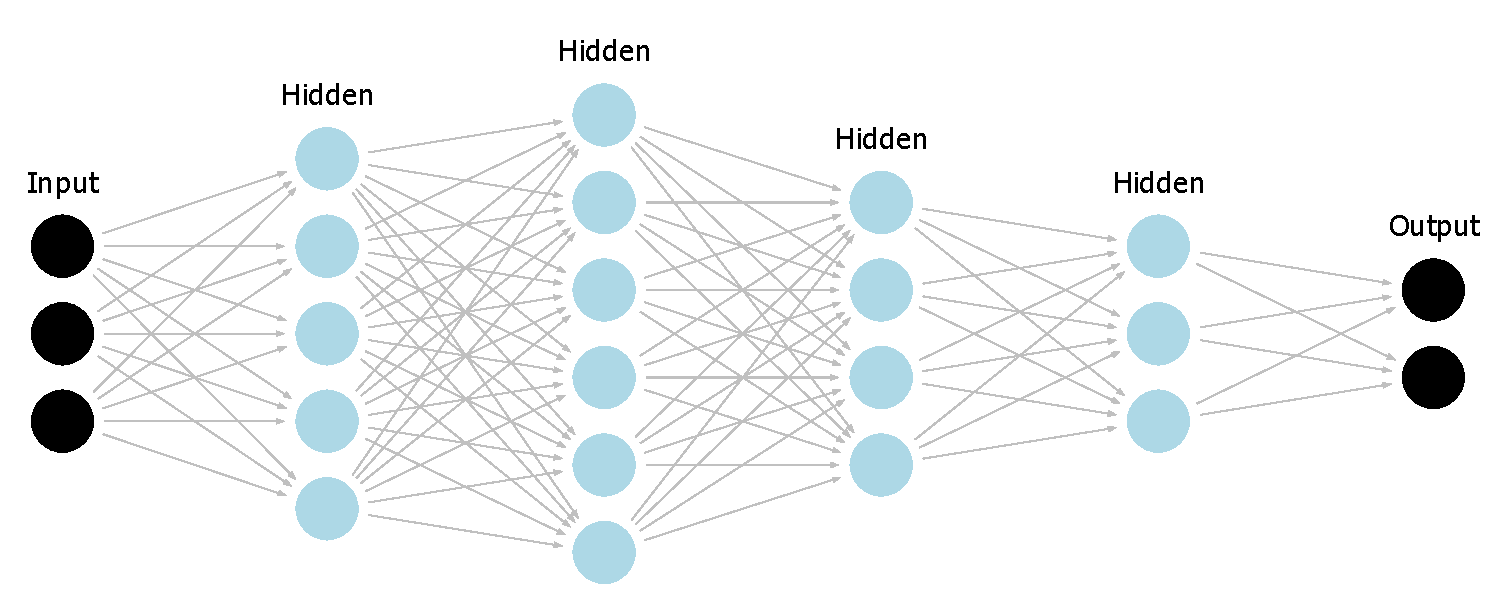
\includegraphics[width=14cm]{deep_nn.pdf}
    \caption[Deep Neural Network]{Deep Neural Network\setcounter{footnote}{0}\footnotemark}
    \label{fig:deep_nn}
\end{figure}
\footnotetext{使用\cite{martisak2018dotnets}绘制}

事实上,神经网络的层数并不是越多越好。在尝试用神经网络解决问题时,可以先从单纯的逻辑回归和浅层神经网络开始,如果其无法解决问题再尝试深层神经网络。

%%%
\subsection{Forward Propagation in a Deep Network}
\index{Forward Propagation}
\textbf{前向传播(Forward Propagation)}是指从输入层开始,逐层计算,直到输出层,得到最终的输出值。在前向传播过程中,对于每一层都已知$A^{[l-1]}$,需要计算$Z^{[l]}$和$A^{[l]}$,计算公式如下:
\begin{align}
    Z^{[l]} &= W^{[l]} A^{[l-1]} + b^{[l]} \\
    A^{[l]} &= g^{[l]}(Z^{[l]})
\end{align}
对于输入层,$A^{[0]} = X$,以此为起点逐层向前计算。在计算完一层后,通常需要把$A^{[l]}$或$Z^{[l]}$存入 \verb|cache|,以便在反向传播时使用,而$W^{[l]}$和$b^{[l]}$从 \verb|parameters| 中读取。

%%%
\subsection{Building Blocks of Deep Neural Networks}
一张图 \ref{fig:blocks_fb} 即可说明。
\begin{figure}[htb!]
    \centering
    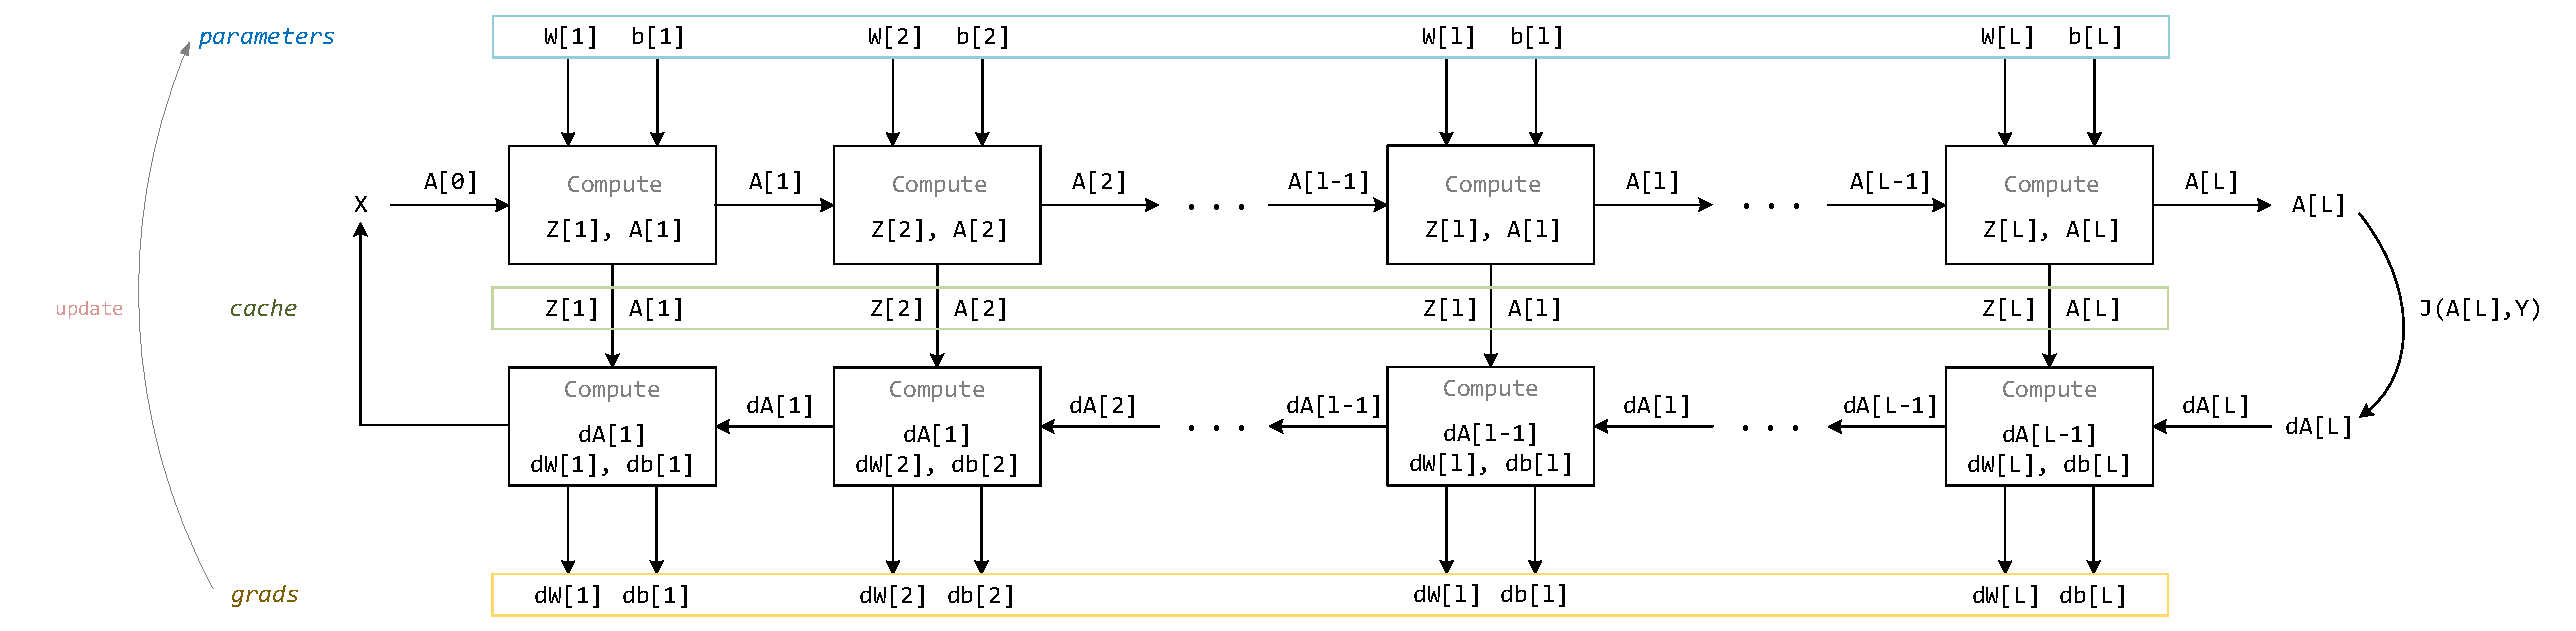
\includegraphics[width=\textwidth]{blocks_fb.pdf}
    \caption{Propagation Blocks}
    \label{fig:blocks_fb}
\end{figure}

一轮迭代包括前向传播和反向传播两个过程,每轮迭代都会不断更新参数$W$和$b$。经过多轮迭代后,可以得到最终的$W$和$b$,然后使用这些参数进行预测。

%%%
\subsection{Parameters vs Hyperparameters}
\textbf{参数(Parameters)}是指神经网络中的$W$和$b$,而\textbf{超参数(Hyperparameters)}是指学习率$\alpha$、迭代次数$T$、神经网络中的层数$L$、每层的神经元数目$n$、激活函数$g$等。

之所以把层数、神经元数目、激活函数等称为超参数,是因为这些参数的值是相对于算法本身而言的,需要人为设定,而不能通过训练得到。在实际应用中,通常需要多次尝试不同的超参数,才能得到较好的结果。
